\documentclass{article}
\usepackage[vietnamese]{babel}
\usepackage{enumitem}
\usepackage{listings}
\usepackage{xcolor}
\usepackage{graphicx}
\usepackage{titlesec}
\usepackage{tabularx}
\usepackage{array}

\setcounter{secnumdepth}{4}
\definecolor{green}{rgb}{0,0.6,0}
\definecolor{gray}{rgb}{0.5,0.5,0.5}
\definecolor{mauve}{rgb}{0.58,0,0.82}

\lstset{frame=tb,
  language=Java,
  aboveskip=3mm,
  belowskip=3mm,
  showstringspaces=false,
  columns=flexible,
  basicstyle={\small\ttfamily},
  numbers=none,
  numberstyle=\tiny\color{gray},
  keywordstyle=\color{blue},
  commentstyle=\color{dkgreen},
  stringstyle=\color{mauve},
  breaklines=true,
  breakatwhitespace=true,
  tabsize=3
}
\begin{document}
\begin{center}
    \textbf{\Large ĐẠI HỌC QUỐC GIA HÀ NỘI}\\
    \textbf{\Large TRƯỜNG ĐẠI HỌC CÔNG NGHỆ}\\
    
    *********************\\
    \vskip 0.5in
    
\includegraphics[scale=1.5]{UETLogo.png}

    \vskip 0.5in
    \textbf{\large KHO DỮ LIỆU}\\
    
    \textbf{\large BÁO CÁO THIẾT KẾ KHO DỮ LIỆU}\\
    
    \vskip 0.3in
    
    \textbf{\large NHÓM 2}\\
    \textbf{\large CHỦ ĐỀ: FINANCIAL SERVICES}\\
\end{center}
\vskip 0.5in
\begin{flushleft}
    \textbf{Giảng viên:} \hspace{0.6cm} Nguyễn Hà Nam\\
    \vskip 0.2in
    \textbf{Sinh viên:} \hspace{1cm}Đặng Quang Huy\\
    \hspace{2.8cm} Lưu Hoàng Nam\\
    \hspace{2.8cm} Hoàng Vũ Duy Anh\\
    \hspace{2.8cm} Nguyên Công Khánh\\
    
\end{flushleft}


\newpage
\section{Giới thiệu bài toán}
\subsection{Đặt vấn đề}

\hspace{0.5cm} Với sự phát triển của cuộc sống hiện đại ngày nay, các dịch vụ tài chính cũng có sự tăng trưởng mạnh mẽ. Trong đó, dịch vụ
cho vay của ngân hàng là dịch vụ tài chính được tin cậy và có khối lượng giao dịch lớn nhất trên thị trường. 
Việc phân tích dữ liệu của cho vay của ngân hàng có thể giúp cho ngân hàng thực hiện các chiến lược hiệu quả
cũng như nắm bắt khách hàng tốt hơn.\\

\subsection{Mô tả bài toán}
\hspace{0.5cm} Trước khi đi vào các vấn đề bài toán, ta sẽ nói về một số khái niệm và quy trình của ngân hàng.
Gói cho vay là một chính sách cho vay đã được định nghĩa sẵn của ngân hàng. 
Các gói cho vay có thời hạn cho vay nhất định (ví dụ 3 tháng, 6 tháng, 12 tháng, ...), 
có thời gian thanh toán định kì (ví dụ sau mỗi một tháng hay một quý phải trả một lần, ...), lãi suất, mục đích cho vay,
cách tính hạn mức cho vay ... Ngoài ra, các khoản vay có thể là vay tín chấp hoặc vay thế chấp.\\

Khách hàng sẽ lựa chọn một trong các gói cho vay. Sau đó cung cấp các thông tin cần thiết cho ngân hàng để xác định hạn mức cho vay, lựa chọn số tiền muốn vay. Sau đố ngân hàng thực hiện liên kết tài khoản của khách hàng với khoản vay và thực hiện việc thu phí định kì
như trong gói vay. Các giao dịch thu nợ sẽ được ngân hàng ghi lại. Khi một khách hàng không có khả năng
trả nợ, khoản nợ đó bị gọi là nợ xấu. Khách hàng bị nợ xấu sẽ gặp nhiều khó khăn khi vay tiền ở tổ chức tài chính khác.\\

\subsection{Các vấn đề cần giải quyết}
Mục đích của ta là xây dựng kho dữ liệu, qua đó giải quyết một số vấn đề sau:
\begin{itemize}
    \setlength\itemsep{0.3em}
    \item Phân tích khối lượng giao dịch của các loại gói vay. 
    \item Nhóm khách hàng mang lại khối lượng và lợi nhuận cho ngân hàng lớn nhất
    \item Nhóm khách hàng thường mấc nợ xấu, trả nợ quá hạn. 
    \item Với các khoản vay đang trong thời gian trả nợ, dự đoán và thống kê các thông tin liên quan.
    \item So sánh sự ảnh hưởng của đại dịch đến từng nhóm khách hàng thông qua phân tích dữ liệu từ trước năm 2019 so với từ sau năm 2019. 
\end{itemize}
\newpage
\section{Thiết kế cơ sở dữ liệu}
\subsection{Thiết kế lược đồ ER}
\subsubsection{Xác định các thực thể}
\begin{itemize}
    \item \textbf{Customer:} Khách hàng
    \item \textbf{Account:} Tài khoản của khách hàng
    \item \textbf{Branch:} Chi nhánh ngân hàng
    \item \textbf{LoanCatergory:} Gói vay
    \item \textbf{Loan:} Khoản vay của khách hàng
    \item \textbf{LoanTransaction:} Bản ghi của các giao dịch liên quan đến khoản vay
\end{itemize}
\subsubsection{Xác định thuộc tính}
\begin{itemize}
    \item \textbf{Customer:}
    \begin{itemize}
        \item \textbf{ID:} Số căn cước công dân của khách hàng.
        \item \textbf{Name:} Tên khách hàngs 
        \item \textbf{Job:} Công việc hiện tại.
        \item \textbf{DOB:} Ngày sinh của khách hàng.
        \item \textbf{Address:} Địa chỉ. 
        \item \textbf{MaritalStatus:} Trạng thái hôn nhân.
        \item \textbf{Income:} Thu nhập hàng tháng.
        
    \end{itemize}
    \item \textbf{Account:}
    \begin{itemize}
        \item \textbf{AccountID:} Mã số tài khoản.
        \item \textbf{Balance:} Số dư hiện tại của tài khoản.
        \item \textbf{CreatedDate:} Ngày tạo tài khoản.
    \end{itemize}
    
    \item \textbf{Branch:}
    \begin{itemize}
        \item \textbf{BranchID:} Mã chi nhánh
        \item \textbf{Address:} Địa chỉ chi nhánh
    \end{itemize}
        
    \item \textbf{LoanCategory:}
    \begin{itemize}
        \item \textbf{CategoryID:} Mã số gói vay.
        \item \textbf{Lifespan:} Thời gian được quy định mà khách hàng cần trả hết số tiền khoản vay.
        \item \textbf{Rate:} Lãi suất cho vay.
        \item \textbf{Purpose:} Mục đích sử dụng vốn vay (vay tiêu dùng, vay kinh doanh).
        \item \textbf{IsSecured:} Khoản vay có tài sản thế chấp hay không.
    \end{itemize}
    
    \item \textbf{Loan:}
    \begin{itemize}
        \item \textbf{LoanID:} Mã số khoản vay
        \item \textbf{AvailableAmount:} Số tiền khách hàng có thể thực hiện vay
        \item \textbf{StartDate:} Ngày bắt đầu cho vay
    \end{itemize}
    
    \item \textbf{LoanTransaction:}
    \begin{itemize}
        \item \textbf{LoanID:} Mã số khoản vay
        \item \textbf{PaidAmount:} Số tiền khách hàng trả cho ngân hàng
        \item \textbf{LoanAmount:} Số tiền ngân hàng cho khách hàng vay
        \item \textbf{Date:} Ngày thực hiện giao dịch
    \end{itemize}
\end{itemize}

\subsubsection{Xác định các quan hệ}
\begin{itemize}
    \item Mỗi Customer có thể sở hữu nhiều Account, biểu diễn bằng quan hệ Has (Có), với tỉ số lực lượng tham gia là 1:n.
    \item Mỗi Branch có thể quản lí nhiều Account, biểu diễn bằng quan hệ Manage(Quản lí), với tỉ số lực lượng tham gia là 1:n.
    \item Mỗi Account được liên kết với một hoặc nhiều Loan, biểu diễn bằng quan hệ Link, với tỉ số lực lượng tham gia là 1:n.
    Account chỉ tham gia bộ phận vào liên kết, trong khi Loan bắt buộc phải Link với ít nhất 1 Account.
    \item Một Loan có loại thuộc một trong các LoanCategory, biểu diễn bằng quan hệ Is, với tỉ số lực lượng tham gia là n:1.
    \item Một Loan bao gồm nhiều LoanTransaction, biểu diễn bằng quan hệ Include, tỉ số lực lượng tham gia là 1:n.
    
\end{itemize}

\subsubsection{Biểu đồ thực thể liên kết}
\begin{center}
    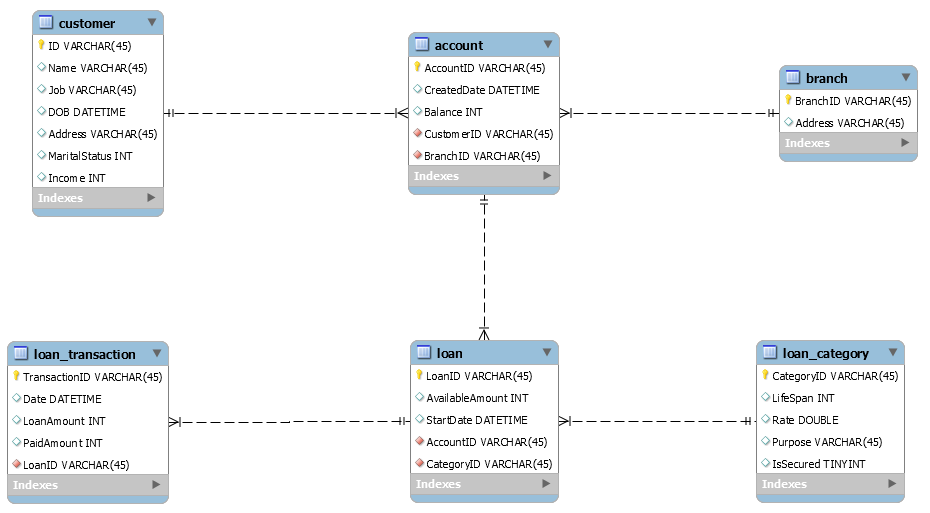
\includegraphics[scale=0.25]{DBDiagram.png}
\end{center}
\subsection{Xây dựng cơ sở dữ liệu}
\subsubsection{Chuyển đổi cơ sở dữ liệu}
Ta xây dựng các bảng với các cột như sau:
\begin{itemize}
    \item \textbf{customer:}
    \begin{itemize}
        \item \textbf{ID:} Khóa chính, kiểu varchar.
        \item \textbf{Name:} Kiểu varchar. 
        \item \textbf{Job:} Kiểu varchar.
        \item \textbf{DOB:} Kiểu datetime.
        \item \textbf{Address:} Kiểu varchar. 
        \item \textbf{MaritalStatus:} Kiểu int, nhận giá trị trong khoảng 0-3 với ý nghĩa như sau:
        \begin{itemize}
            \item 0: độc thân.
            \item 1: kết hôn.
            \item 2: li thân.
            \item 3: li dị. 
        \end{itemize}
        \item \textbf{Income:} Kiểu int.
        
    \end{itemize}
    \item \textbf{account:}
    \begin{itemize}
        \item \textbf{AccountID:} Khóa chính, kiểu varchar.
        \item \textbf{Balance:} Kiểu int.
        \item \textbf{CreatedDate:} Ngày tạo tài khoản.
        \item \textbf{CustomerID:} Khóa ngoại đến bảng customer.
        \item \textbf{BranchID:} Khóa ngoại đến bảng branch.
    \end{itemize}
    
    \item \textbf{branch:}
    \begin{itemize}
        \item \textbf{BranchID:} Khóa chính, kiểu varchar.
        \item \textbf{Address:} Kiểu varchar.
    \end{itemize}
        
    \item \textbf{loan category:}
    \begin{itemize}
        \item \textbf{CategoryID:} Khóa chính, kiểu varchar.
        \item \textbf{Lifespan:} Kiểu int thể hiện số ngày cho vay.
        \item \textbf{Rate:} Kiểu double.
        \item \textbf{Purpose:} Kiểu varchar.
        \item \textbf{IsSecured:} Kiểu boolean.
    \end{itemize}
    
    \item \textbf{loan:}
    \begin{itemize}
        \item \textbf{LoanID:} Khóa chính, kiểu varchar.
        \item \textbf{AvailableAmount:} Kiểu int.
        \item \textbf{StartDate:} Kiểu datetime.
        \item \textbf{AccountID:} Khóa ngoại đến bảng account.
        \item \textbf{CategoryID:} Khóa ngoại đến bảng loan category.
    \end{itemize}
    
    \item \textbf{loan transaction:}
    \begin{itemize}
        \item \textbf{LoanID:} Khóa chính, kiểu varchar.
        \item \textbf{PaidAmount:} Kiểu int.
        \item \textbf{LoanAmount:} Kiểu int.
        \item \textbf{Date:} Kiểu datetime.
        \item \textbf{LoanID:} Khóa ngoại đến bảng loan.
    \end{itemize} 
\end{itemize}
\subsubsection{Lược đồ cơ sở dữ liệu}
\begin{center}
    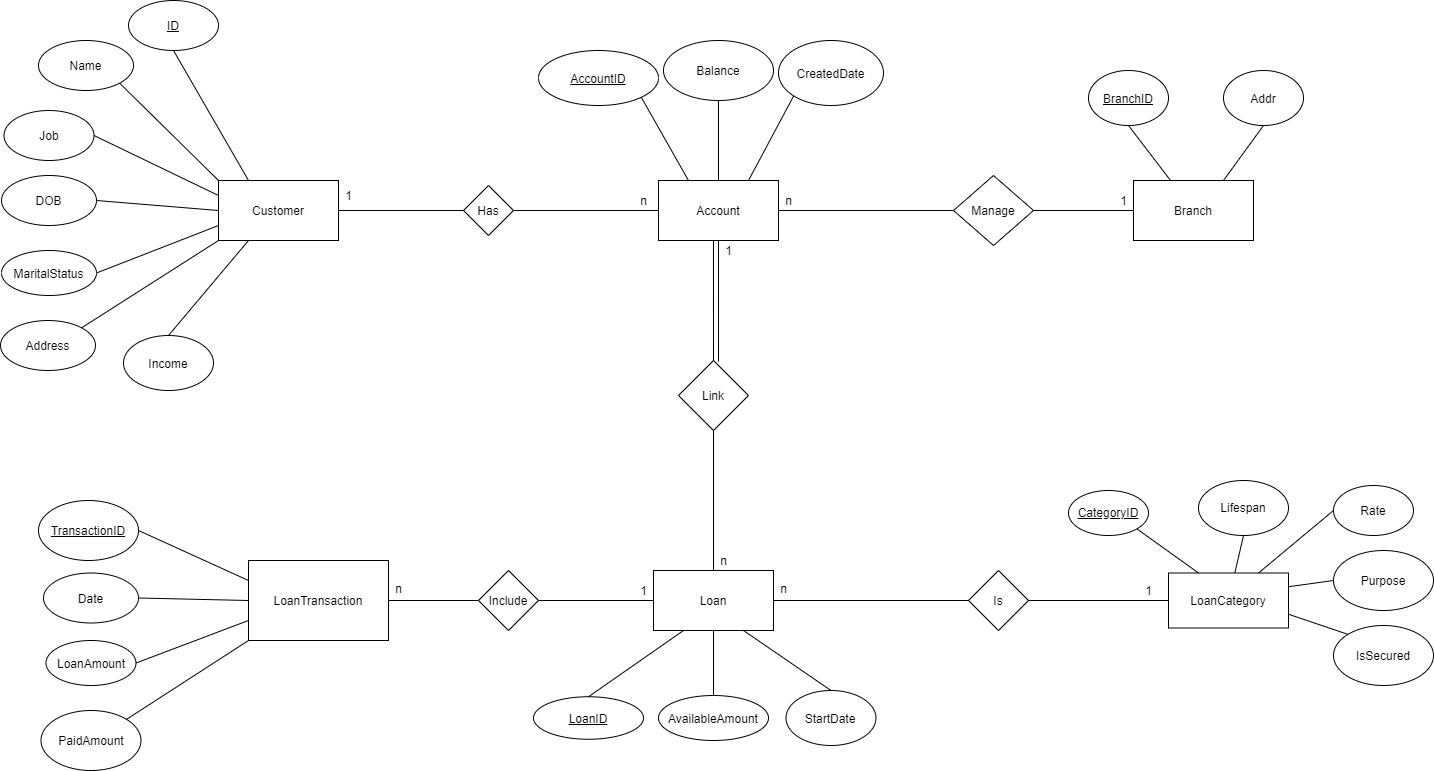
\includegraphics[scale=0.5]{ERDiagram.jpg}
\end{center}

\subsection{Thu thập dữ liệu và thêm dữ liệu vào cơ sở dữ liệu}
Việc cài đặt được thực hiện trên hệ quản trị cơ sở dữ liệu quan hệ MySQL server.

\section{Xây dựng kho dữ liệu}
\subsection{Chuyển đổi cơ sở dữ liệu sang kho dữ liệu}
\subsubsection{Lựa chọn quy trình nghiệp vụ}
Quy trình nghiệp vụ mà ta muốn cải tiến là nghiệp vụ cho vay.
\subsubsection{Định nghĩa mức độ chi tiết}
Mỗi dòng của bảng fact tương ứng với một giao dịch liên quan đến khoản vay.
\subsubsection{Xác định các dimensions}
\begin{itemize}
    \item \textbf{date dimension.} Dimension biểu diễn thời gian chính xác đến ngày, có các thuộc tính sau:
    \begin{itemize}
        \item \textbf{DateKey:} Mã ngày.
        \item \textbf{Date:} Thể hiện giá trị ngày, kiểu int, nhận giá trị 1 đến 31.
        \item \textbf{Month:} Thể hiện giá trị tháng, kiểu int, nhận giá trị từ 1 đến 12.
        \item \textbf{Quarter:} Thể hiện giá trị quý, kiểu int, nhận giá trị từ 1 đến 4.
        \item \textbf{Year:} Thể hiện giá trị năm, kiểu int.
    \end{itemize}
    \item \textbf{customer dimension}. Dimension biểu diễn thông tin của khách hàng, có các thuộc tính sau:
    \begin{itemize}
        \item \textbf{CustomerKey:} Mã khách hàng. Kiểu varchar.
        \item \textbf{Name:} Tên khách hàng. Kiểu varchar.
        \item \textbf{DOB:} Ngày sinh của khách hàng. Kiểu datetime.
        \item \textbf{Province:} Tên tỉnh thành khách hàng đang sống.
        \item \textbf{City:} Thành phố nơi khách hàng đang sống.
        \item \textbf{Street:} Tên đường nơi khách hàng đang sống.
    \end{itemize}
    \item \textbf{customer demographic dimension}. Dimension biểu diễn thông tin thường xuyên thay đổi của khách hàng. 
    \begin{itemize}
        \item \textbf{CustomerDemographicKey:} Khóa chính của bảng. Kiểu varchar.
        \item \textbf{AgeBand:} Khoảng tuổi của khách hàng. Giá trị int. 
        \item \textbf{IncomeBand:} Khoảng thu nhập của khách hàng. Kiểu int.
        \item \textbf{MaritalStatus:} Trạng thái hôn nhân. Kiểu int.
        \item \textbf{IsEmployed:} Đang có công việc hay không. Kiểu boolean.
    \end{itemize}
    \item \textbf{branch dimension}. Dimension biểu diễn thông tin chi nhánh nơi khách hàng nộp hồ sơ khoản vay.
    \begin{itemize}
        \item \textbf{BranchKey:} Mã chi nhánh. Kiểu varchar.
        \item \textbf{Province:} Tên tỉnh thành. Kiểu varchar.
        \item \textbf{City:} Tên thành phố. Kiểu varchar.
        \item \textbf{Street:} Tên đường. Kiểu varchar.
    \end{itemize}
    \item \textbf{loan category dimension:}
    \begin{itemize}
        \item \textbf{CategoryKey:} Mã gói vay. Kiểu varchar.
        \item \textbf{Lifespan:} Kì hạn vay. Kiểu int.
        \item \textbf{Rate:} Lãi suất cho vay. Kiểu double.
        \item \textbf{Purpose:} Mục đích sử dụng vốn. Kiểu varchar.
        \item \textbf{IsSecured:} Khoản vay có tài sản thế chấp không. Kiểu boolean.
    \end{itemize}
    
    \item \textbf{loan started date dimension:}
    \begin{itemize}
        \item \textbf{LoanStartedDateKey:} Mã số ngày bắt đầu vay.
        \item \textbf{LoanStartedDate:} Ngày bắt đầu vay.
        \item \textbf{LoanStartedMonth:} Tháng bắt đầu vay.
        \item \textbf{LoanStartedYear:} Năm bắt đầu vay.
        \item \textbf{LoanStartedQuater:} Quý bắt đầu vay.
    \end{itemize}
    
    \item \textbf{loan dimension:} 
    \begin{itemize}
        \item \textbf{LoanKey:} Mã khoản vay
        \item \textbf{AvailableAmount:} Số tiền vay khả dụng của khách hàng.
        \item \textbf{LoanStartedDateKey:} Khóa ngoại đến loan started date dimension. 
    \end{itemize}
\end{itemize}
\subsubsection{Xác định facts}
    Bảng fact cung cấp thông tin về lượng tiền vay và lượng tiền. 
    \textbf{loan transaction fact}:
    \begin{itemize}
        \item \textbf{DateKey:} Khóa ngoại đến DateDimension.
        \item \textbf{BranchKey:} Khóa ngoại đến BranchDimension.
        \item \textbf{CategoryKey:} Khóa ngoại đến CategoryDimension.
        \item \textbf{CustomerKey:} Khóa ngoại đến Customer.
        \item \textbf{CustomerDemographicKey:} Khóa ngoại đến CustomerDemographic.
        \item \textbf{RepaidAmount:} Số tiền trả lãi cho ngân hàng. Kiểu INT.
        \item \textbf{LoanAmount:} Lượng tiền khách hàng vay trong tháng.

    \end{itemize}
    
\subsubsection{Mô hình kho dữ liệu.}
\begin{center}
    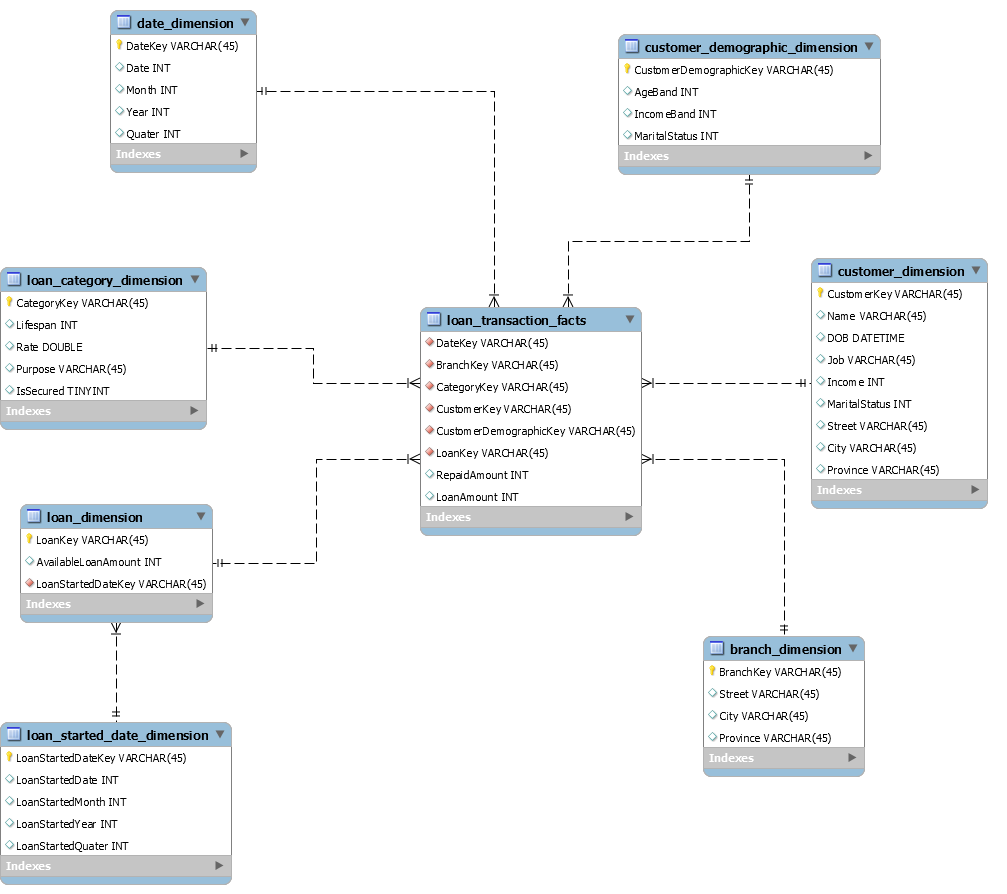
\includegraphics[scale=0.4]{DatawarehouseSchema.png}
\end{center}
\newpage
\section{Khai thác dữ liệu}
\subsection{Các câu hỏi mang tính thống kê.}
\subsection{Các câu hỏi dự báo.}

\section{Trích dân}

\end{document}